\chapter{弯曲流形}
\label{chap6}

\section{微分流形,张量}
\label{sec6.1}

\subsection*{流形}

\subsection*{微分结构}
我们只考虑“微分流形”(differentiable manifolds),它们是连续且可微的空间。粗略地说,微分流形的每一点的邻域都可定义从该邻域到欧几里得空间的光滑映射,该映射保证标量函数的导数在那一点不变。球面是处处可微的,而锥面除了顶点以外处处可微。物理学用到的流形基本上都是几乎处处可微的,GR的弯曲流形就是如此。

可微性的条件直接意味着可以定义1形式与向量。也就是说,在流形上的某个坐标系中,集合$\{ \phi_{, \alpha} \}$的元素是1形式$\trd \phi$的分量;而集合$\{ a \phi_{, \alpha} + b \psi_{, \alpha} \}$(其中$a, b$是函数)也是1形式场。类似的,任何曲线(带有参数,例如$\lambda$)具有切向量$\vec{V}$,它定义为将1形式$\trd \phi$变成“标量场沿该曲线的导数$\rd \phi / \rd \lambda$”的线性函数:
\begin{equation}
    \langle \trd \phi, \vec{V} \rangle = \vec{V} (\trd \phi) = \nabla_{\vec{V}} \phi = \frac{\rd \phi}{\rd \lambda}.
\label{equ6.1}
\end{equation}
向量的线性组合也是向量。利用上面定义的向量和1形式,可以定义各种$\binom{M}{N}$型张量,就像SR里定义的那样。由于目前尚未钦点任何$\binom{0}{2}$张量为度规,因此向量与1形式之间还没有对应关系。不过其它内容与之前讨论的SR情形、极坐标系相同。这些内容都来自于微分,因此所有张量的集合称为流形的“微分结构 (differential structure)”的一部分。我们不会经常使用这个术语。


\subsection*{回顾}

\section{Riemannian流形}
\label{sec6.2}
目前为止尚未在流形中引入度规。在一些问题的流形中,度规是不必要或不常用的。但是对GR而言,度规绝对是最基本的,因为就像SR那样,度规描述了钟的走时与两点的距离。一个微分流形配上一个被选召为度规的、对称的$\binom{0}{2}$张量场$\bm{g}$,称为Riemannian流形(黎曼流形)。\textit{严格来说,只有当度规是正定的——即$\forall\, \vec{V} \neq 0, \bm{g} (\vec{V}, \vec{V}) > 0$——才叫做Riemannian流形;SR与GR那样的不定度规情况叫做pseudo-Riemannian(伪黎曼流形)。不过作为一本物理书我们并不区分统统称为Riemannian流形。} 选出一个度规意味着在流形上“添加”某种结构,理解这一点很关键,之后会看到这个度规完全定义了流形的曲率。因此,选定一个度规$\bm{g}$之后,流形具有了一种曲率(例如,球面),而选择另一个度规$\bm{g}'$流形具有另一种曲率(例如,旋转椭球面)。“原始的”微分流形自身是一团无定形的点的集合,并且局域地相似于欧几里得空间中的点的排布,其中的距离与形状并未指定。给定了度规$\bm{g}$就赋予了流形以特定形状,后面就会看到。从现在开始,我们讨论的对象是Riemannian流形,其上的每一点都定义了度规$\bm{g}$。

\textit{为了内容完整,我们指出,可以不利用度规来定义流形曲率的概念(称为“仿射 (affine)”流形)。有些文献用采用这种方法,但是度规在GR中的地位是基本的,因此我们利用度规定义流形曲率。}


\subsection*{度规,局域平直性}
自然,度规提供了每一点的向量与1形式之间的映射。因此,给定向量场$\vec{V} (\mathcal{P})$(这个符号意味着$\vec{V}$取决于位置$\mathcal{P}$,$\mathcal{P}$是流形中的任一点),它唯一对应于1形式场$\tilde{V} (\mathcal{P}) = \bm{g} (\vec{V} (\mathcal{P}), \ )$。这个映射必须是可逆的\sout{画外音:看不出来……},因此$\tilde{V} (\mathcal{P})$也对应唯一的$\vec{V} (\mathcal{P})$。$\bm{g}$的分量记作$g_{\alpha \beta}$;分量矩阵的逆矩阵记作$g^{\alpha \beta}$。度规可以升降指标,就像SR中的那样:
\[
    V_\alpha = g_{\alpha \beta} V^\beta.
\]
一般的$\{ g_{\alpha \beta} \}$是坐标的复杂函数,因此在一般的坐标系中,向量与1形式分量,例如$V^0$与$V_0$,一般没有简单的关系。

要研究一般的弯曲流形就要在一般的坐标系中考虑问题。SR只在Lorentz系(惯性系)中讨论(因为简单),但是引力使得全局惯性系不存在,因此我们得考虑所有的(一般性的)坐标系,以及所有的(一般性的)非奇异坐标变换。\textit{非奇异性在\ref{sec5.2}节介绍过,它意味着变换矩阵$\Lambda\indices{^{\alpha'}_\beta} \equiv \partial x^{\alpha'} / \partial x^\beta$可逆。} 根据定义,度规分量矩阵$(g_{\alpha \beta})$是对称的,线性代数的一条重要定理(见第\ref{chap6}章习题3)告诉我们,对于任意对称矩阵$(g_{\alpha' \beta'})$,总可以找到变换矩阵将$(g_{\alpha' \beta'})$化为对角元是$+1, -1$或0的对角矩阵,且$+1$的数量等于矩阵$(g_{\alpha' \beta'})$的正特征值的个数、$-1$的数量等于负特征值个数。故而,如果一开始选择$\bm{g}$的分量矩阵具有3个正特征值、1个负特征值,则总可以找到变换矩阵$\Lambda\indices{^{\alpha'}_\beta}$使得度规分量变换为:
\begin{equation}
    (g_{\alpha' \beta'}) = 
    \begin{pmatrix}
        -1 & 0 & 0 & 0 \\
        0 & 1 & 0 & 0 \\
        0 & 0 & 1 & 0 \\
        0 & 0 & 0 & 1
    \end{pmatrix}
    \equiv (\eta_{\alpha \beta}).
\label{equ6.2}
\end{equation}
今后,$\eta_{\alpha \beta}$ \textit{专指}上式中的矩阵,也就是SR的度规。

有两点重要内容必须指出。第一,只有$(g_{\alpha \beta})$选为3个正特征值、1个负特征值的时候,\eqref{equ6.2}式才可能。\eqref{equ6.2}式矩阵的对角元素之和称为度规的\textit{号差 (signature)},SR与GR的度规号差都是$+2$。因此,之前我们论述过,在任意事件处总可以构造一个\textit{局域}惯性系,方程\eqref{equ6.2}是这个物理命题的数学表述,亦即,该点的度规总可以变换为$\eta_{\alpha \beta}$。反过来,这意味着一个描述有引力时空的度规的号差必须是$+2$。

第二,\eqref{equ6.2}式对应的变换矩阵$\Lambda\indices{^{\alpha'}_\beta}$也许\textit{并非}坐标变换。也就是说,集合$\{ \tilde{\omega}^{\alpha'} = \Lambda\indices{^{\alpha'}_\beta} \trd x^\beta \}$也许不是坐标基。根据前面对非坐标基的讨论,$\Lambda\indices{^{\alpha'}_\beta}$只有当\eqref{equ5.95}式成立时才是坐标变换:
\[
    \frac{\partial \Lambda\indices{^{\alpha'}_\beta}}{\partial x^\gamma} = \frac{\partial \Lambda\indices{^{\alpha'}_\gamma}}{\partial x^\beta}.
\]

这在一般的引力场中不能成立,否则就意味着存在\eqref{equ6.2}式处处成立的坐标系——全局惯性系了。不过,既然可以使\eqref{equ6.2}式在$\mathcal{P}$点成立,那么也可以找到坐标系使得\eqref{equ6.2}式在$\mathcal{P}$点的邻域“近似”成立。这体现在如下的定理中,该定理的证明(相当长)见本节最后。对于流形上的任一点$\mathcal{P}$,可以找到原点为$\mathcal{P}$点的坐标系$\{ x^\alpha \}$,在该坐标系中:
\begin{equation}
    g_{\alpha \beta} (x^\mu ) = \eta_{\alpha \beta} + 0 [(x^\mu)^2].
\label{equ6.3}
\end{equation}
这意味着,$\mathcal{P}$点附近的度规近似是SR的度规,相差坐标的二阶量。今后称这种坐标系为“\textbf{局域Lorentz系}”或“\textbf{局域惯性系} (local inertial frames, \textbf{LIF})”。方程\eqref{equ6.3}可以表示为更精确的形式:
\begin{shaded}
\begin{align}
    g_{\alpha \beta} (\mathcal{P}) &= \eta_{\alpha \beta} \quad \forall\, \alpha, \beta; \label{equ6.4} \\
    \frac{\partial}{\partial x^\gamma} g_{\alpha \beta} (\mathcal{P}) &= 0 \quad \forall\, \alpha, \beta, \gamma; \label{equ6.5}
\end{align}
\end{shaded}
但是在一般情况下
\begin{shaded}
\begin{equation*}
    \frac{\partial^2}{\partial x^\gamma \partial x^\mu} g_{\alpha \beta} (\mathcal{P}) \neq 0
\end{equation*}
\end{shaded}
在弯曲流形中,上式至少对某些$\alpha, \beta, \gamma, \mu$成立。

局域惯性系的存在性等价于弯曲空间中的任一点存在“相切”的平坦空间。平直时空中,自由粒子的世界线是直线;方程\eqref{equ6.5}中弯曲时空度规的一阶导数项为零意味着,弯曲时空中的自由粒子沿着在局域惯性系中的“局域直”的线运动。由于物理学方程在平直时空中最简单,而按照\ref{sec6.1}节总结的规律,只要在局域惯性系写出张量等式的方程,则该方程在任意坐标系都有效,因此局域惯性系十分有用。别忘了定理的证明在本节最后,尽管比较长,但是它值得研究。

\subsection*{长度与体积}
度规定义了曲线的长度。将曲线上的无穷小位移向量记作$\rd \vec{x}$,则$\rd \vec{x}$长度的平方$\rd s^2 = g_{\alpha \beta} \rd x^\alpha \rd x^\beta$(回顾一下,前面称之为度规的\textit{线元})。对它的绝对值开平方就是长度:$\rd \ell \equiv |  g_{\alpha \beta} \rd x^\alpha \rd x^\beta |^{1/2}$,再进行积分:
\begin{align}
    \ell &= \int_{\text{沿曲线}} | g_{\alpha \beta} \rd x^\alpha \rd x^\beta | ^{1/2} \label{equ6.6} \\
    &= \int_{\lambda_0}^{\lambda_1} \left| g_{\alpha \beta} \frac{\rd x^\alpha}{\rd \lambda} \frac{\rd x^\beta}{\rd \lambda} \right|^{1/2} \, \rd \lambda, \label{equ6.7}
\end{align}
其中$\lambda$是曲线的参数(端点处的参数值为$\lambda_0, \lambda_1$)。由于曲线的切向量$\vec{V}$的分量为$V^\alpha = \rd x^\alpha / \rd \lambda$,上式可写为:
\begin{shaded}
\begin{equation}
    \ell = \int_{\lambda_0}^{\lambda_1} | \vec{V} \cdot \vec{V} |^{1/2} \, \rd \lambda,
\label{equ6.8}
\end{equation}
\end{shaded}
这就是任意曲线的长度。

在对时空区域进行积分时,计算体积十分重要。这里的“体积”是指四维体积元,它出现于\ref{sec4.4}节Gauss定律的积分中。局域惯性系的无穷小四维体元的四维体积为$\rd x^0\, \rd x^1\, \rd x^2\, \rd x^3$,其中$\{ x^\alpha \}$是原点在指定点的局域惯性系,满足方程\eqref{equ6.3}。在\textit{任意}坐标系$\{ x^{\alpha'}\}$中,根据多变量微积分的知识可得:
\begin{equation}
    \rd x^0\, \rd x^1\, \rd x^2\, \rd x^3 = \frac{\partial (x^0, x^1, x^2, x^3)}{\partial (x^{0'}, x^{1'}, x^{2'}, x^{3'}) } \rd x^{0'}\, \rd x^{1'}\, \rd x^{2'}\, \rd x^{3'},
\label{equ6.9}
\end{equation}
其中$\partial (\ ) / \partial (\ )$是从$\{ x^{\alpha'} \}$到$\{ x^\alpha \}$的变换的Jacobian(雅可比行列式),在\ref{sec5.2}节定义过:
\begin{align}
    \frac{\partial (x^0, x^1, x^2, x^3)}{\partial (x^{0'}, x^{1'}, x^{2'}, x^{3'}) } &= \det \begin{pmatrix}
        \partial x^0 / \partial x^{0'} & \partial x^0 / \partial x^{1'} & \dots \\
        \partial x^1 / \partial x^{0'} & \ & \  \\
        \vdots &&
    \end{pmatrix} \notag \\
    &= \det (\Lambda\indices{^\alpha_{\beta'}}). \label{equ6.10}
\end{align}
计算Jacobian的过程相当繁琐,不过利用度规可以简化计算过程。度规分量变换的矩阵形式为
\begin{equation}
    (g) = (\Lambda) (\eta) (\Lambda)^T,
\label{equ6.11}
\end{equation}
其中$(g)$表示矩阵$g_{\alpha \beta}$,$(\eta)$表示$\eta_{\alpha \beta}$,等等。符号$T$表示矩阵转置。上式取行列式:
\begin{equation}
    \det (g) = \det (\Lambda) \, \det (\eta) \, \det (\Lambda^T).
\label{equ6.12}
\end{equation}
转置矩阵的行列式与原矩阵相等:
\begin{equation}
    \det (\Lambda) = \det (\Lambda^T),
\label{equ6.13}
\end{equation}
而根据\eqref{equ6.2}可得
\begin{equation}
    \det (\eta) = -1.
\label{equ6.14}
\end{equation}
综上,
\begin{equation}
    \det (g) = - [\det (\Lambda)]^2.
\label{equ6.15}
\end{equation}
引入记号
\begin{equation}
    g := \det( g_{\alpha' \beta'}),
\label{equ6.16}
\end{equation}
这样方程\eqref{equ6.15}可以写为
\begin{equation}
    \det (\Lambda\indices{^\alpha_{\beta'}}) = (-g)^{1/2}.
\label{equ6.17}
\end{equation}
从而,根据\eqref{equ6.9}式可得:
\begin{shaded}
\begin{align}
    \rd x^0\, \rd x^1\, \rd x^2\, \rd x^3 &= \big[ -\det (g_{\alpha' \beta'}) \big]^{1/2} \, \rd x^{0'}\, \rd x^{1'}\, \rd x^{2'}\, \rd x^{3'} \notag \\
    &= (-g)^{1/2} \, \rd x^{0'}\, \rd x^{1'}\, \rd x^{2'}\, \rd x^{3'}. \label{equ6.18}
\end{align}
\end{shaded}
这个结果非常有用。这个式子的推导思路也很重要,因为这是第一个利用局域惯性系将平直时空的结果推广到弯曲时空的例子,之后会经常利用这种思路。本例从局域惯性系的体元$\rd x^0\, \rd x^1\, \rd x^2\, \rd x^3 = \rd^4 x$出发,由于给定点附近的时空邻域和Minkowski空间相同,因此这个体元就是可以由时钟与尺子测量的物理量。接着我们导出了在任意坐标系$\{ x^{\mu'} \}$的体元表达式\eqref{equ6.18},$(-g)^{1/2} \rd^4 x'$,这就是弯曲时空中任意坐标系的任一点的物理体积元,我们称之为\textit{固有体元 (proper volume element)}。

度规出现在固有体元里,这是在意料之中的,因为度规测量长度。任意坐标系的$\rd^4 x$乘以$(-g)^{1/2}$就得到的真实的,或者说\textit{固有的(proper)}体元。

这里应该举个三次元欧几里得空间的例子,由于该空间的度规是正定的(\eqref{equ6.14}的对应结果是$+1$),因此固有体元应该乘以$(g)^{1/2}$。球坐标系的线元$\rd \ell^2 = \rd r^2 + r^2 \rd \theta^2 + r^2 \sin^2 \theta \rd \phi^2$,因此度规是
\begin{equation}
    (g_{ij}) = 
    \begin{pmatrix}
        1 & 0 & 0 \\
        0 & r^2 & 0 \\
        0 & 0 & r^2 \sin^2 \theta
    \end{pmatrix}.
\label{equ6.19}
\end{equation}
度规行列式等于$r^4 \sin^2 \theta$,所以固有体元$(g)^{1/2} \, \rd^3 x'$等于
\begin{equation}
    r^2 \sin \theta \rd r \rd \theta \rd \phi,
\label{equ6.20}
\end{equation}
这就是人们熟悉的极坐标系的体积元。

\subsection*{局域平直性定理的证明}
记$\{ x^\alpha \}$是任意坐标系,$\{ x^{\alpha'}\}$是局域惯性系:它在所考虑的$\mathcal{P}$点附近简化为惯性系(四维时空流形中的点就是一个事件)。这两个坐标系之间的坐标变换为:
\begin{align}
    x^\alpha &= x^\alpha (x^{\mu'}), \label{equ6.21} \\
    \Lambda\indices{^\alpha_{\mu'}} &= \partial x^\alpha / \partial x^{\mu'}. \label{equ6.22}
\end{align}
将$\Lambda\indices{^\alpha_{\mu'}}$在$\mathcal{P}$点(该点的坐标是$x_0^{\mu'}$)附近作Taylor展开,其中$\vec{x}$是$\mathcal{P}$点附近的一点:
\begin{align}
    \Lambda\indices{^\alpha_{\mu'}} (\vec{x}) =& \Lambda\indices{^\alpha_{\mu'}} (\mathcal{P}) + (x^{\gamma'} - x_0^{\gamma'}) \frac{\partial \Lambda\indices{^\alpha_{\mu'}}}{\partial x^{\gamma'}} (\mathcal{P}) \notag \\
    &+ \frac{1}{2} (x^{\gamma'} - x_0^{\gamma'}) (x^{\lambda'} - x_0^{\lambda'}) \frac{ \partial^2 \Lambda\indices{^\alpha_{\mu'}} }{ \partial x^{\lambda'} \partial x^{\gamma'} } (\mathcal{P}) + \dots , \notag \\
    =& \Lambda\indices{^\alpha_{\mu'}}\bigg|_{\mathcal{P}} + (x^{\gamma'} - x_0^{\gamma'} ) \frac{ \partial^2 x^\alpha }{ \partial x^{\gamma'} \partial x^{\mu'} } \bigg|_{\mathcal{P}} \notag \\
    &+ \frac{1}{2} (x^{\gamma'} - x_0^{\gamma'})(x^{\lambda'} - x_0^{\lambda'}) \frac{ \partial^3 x^\alpha }{ \partial x^{\lambda'} \partial x^{\gamma'} \partial x^{\mu'} } \bigg|_{\mathcal{P}} + \dots. \label{equ6.23}
\end{align}
将度规进行同样的展开:
\begin{align}
    g_{\alpha \beta} (\vec{x}) =& g_{\alpha \beta} \bigg|_{\mathcal{P}} + (x^{\gamma'} - x_0^{\gamma'}) \frac{ \partial g_{\alpha \beta} }{ \partial x^{\gamma'} } \bigg|_{\mathcal{P}} \notag \\
    & + \frac{1}{2} (x^{\gamma'} - x_0^{\gamma'}) (x^{\lambda'} - x_0^{\lambda'}) \frac{\partial^2 g_{\alpha \beta}}{\partial x^{\lambda'} \partial x^{\gamma'}} \bigg|_{\mathcal{P}} + \dots. \label{equ6.24}
\end{align}
将以上两个\sout{两坨}方程带入度规的变换式当中:
\begin{equation}
    g_{\mu' \nu'} = \Lambda\indices{^\alpha_{\mu'}} \Lambda\indices{^\beta_{\nu'}} g_{\alpha \beta},
\label{equ6.25}
\end{equation}
可得:
\begin{align}
    g_{\mu' \nu'} (\vec{x}) =& \Lambda\indices{^\alpha_{\mu'}} \bigg|_{\mathcal{P}} \, \Lambda\indices{^\beta_{\nu'}} \bigg|_{\mathcal{P}} \, g_{\alpha \beta} \bigg|_{\mathcal{P}} \notag \\
    & + (x^{\gamma'} - x_0^{\gamma'}) \Bigg[ \Lambda\indices{^\alpha_{\mu'}} \bigg|_{\mathcal{P}}\, \Lambda\indices{^\beta_{\nu'}} \bigg|_{\mathcal{P}} \, g_{\alpha \beta, \gamma'} \bigg|_{\mathcal{P}} \notag \\
    & + \Lambda\indices{^\alpha_{\mu'}} \bigg|_{\mathcal{P}}\, g_{\alpha \beta} \bigg|_{\mathcal{P}} \, \frac{ \partial^2 x^\beta }{ \partial x^{\gamma'} \partial x^{\nu'} } \bigg|_{\mathcal{P}}  \notag \\
    & + \Lambda\indices{^\beta_{\nu'}} \bigg|_{\mathcal{P}} \, g_{\alpha \beta} \bigg|_{\mathcal{P}} \, \frac{ \partial^2 x^\alpha }{ \partial x^{\gamma'} \partial x^{\mu'} } \bigg|_{\mathcal{P}} \Bigg] \notag \\
    & + \frac{1}{2} (x^{\gamma'} - x_0^{\gamma'}) (x^{\lambda'} - x_0^{\lambda'}) \big[ \dots \big], \label{equ6.26} 
\end{align}
我们不知道坐标变换\eqref{equ6.21}式的具体形式,但是可以通过Taylor展开来定义它,为此首先来计算自由变量的个数。

\begin{itemize}
\item 变换矩阵$\Lambda\indices{^\alpha_{\mu'}}$有16个指标,它们都对应自由变量。
\item 数组$\{ \partial^2 x^\alpha / ( \partial x^{\gamma'} \partial x^{\mu'} ) \big|_{\mathcal{P}} \}$有$4 \times 10 = 40$个自由指标(并非$4 \times 4 \times 4$个,因为指标$\gamma'$与$\mu'$\textit{对称})。
\item 数组$\{ \partial^3 x^\alpha / ( \partial x^{\lambda'} \partial x^{\gamma'} \partial x^{\mu'} ) \big|_{\mathcal{P}} \}$有$4 \times 20 = 80$个自由变量,因为可以\textit{任意更换}指标$\lambda', \gamma', \mu'$的顺序,这种对称性导致一个固定的$\alpha$只对应20个独立变量。\textit{这种三个指标的对称性的独立变量数的一般结论是$n ( n+1) (n+2) / 3!$,其中$n$是每个指标可能取值的个数,对于我们的情况是$n = 4$.}
\item 另一方面,$g_{\alpha \beta} \big|_{\mathcal{P}}, g_{\alpha \beta, \gamma'} \big|_{\mathcal{P}}, g_{\alpha \beta, \gamma' \mu'} \big|_{\mathcal{P}}$都是最初给定的,它们分别具有$10, 10\times4 = 40, 10 \times 10 = 100$个独立分量。
\end{itemize}
第一个问题是,是否可以满足方程\eqref{equ6.4}:
\begin{equation}
    g_{\mu' \nu'} \bigg|_{\mathcal{P}} = \eta_{\mu' \nu'} \ \text{?}
\label{equ6.27}
\end{equation}
上式可以写为
\begin{equation}
    \eta_{\mu' \nu'} = \Lambda\indices{^\alpha_{\mu'}}\bigg|_{\mathcal{P}} \, \Lambda\indices{^\beta_{\nu'}} \bigg|_{\mathcal{P}} \, g_{\alpha \beta} \bigg|_{\mathcal{P}}.
\label{equ6.28}
\end{equation}
根据对称性,上式对应10个独立方程。我们有16个自由的$\Lambda\indices{^\alpha_{\mu'}}\big|_{\mathcal{P}}$来满足这些方程,因此这些方程是可以解出的,并且留下了6个$\Lambda\indices{^\alpha_{\mu'}}\big|_{\mathcal{P}}$尚未确定,这余下的6个变量对应于保证度规$\eta_{\mu' \nu'}$不变的Lorentz变换的自由度。也就是说,可以对坐标系进行绕某个方向(确定该方向需要2个参数)的转轴旋转角度$\theta$(1个参数)的速度为$\bm{v}$(含有3个自由参数)的推动(boost)变换,这就给出了$\Lambda\indices{^\alpha_{\mu'}} \big|_{\mathcal{P}}$的6个自由度,局域惯性系经过这种变换还是惯性系。

下一个问题是,是否可以安排\eqref{equ6.26}式中$\partial \Lambda\indices{^\alpha_{\mu'}} / \partial x^{\gamma'} \big|_{\mathcal{P}}$(它具有40个自由变量),使得方程\eqref{equ6.5}:
\begin{equation}
    g_{\alpha' \beta' , \mu'} \bigg|_{\mathcal{P}} = 0.
\label{equ6.29}
\end{equation} 
的40个独立方程成立?

既然是40个方程、40个未知数,那么答案是“可以”,不多不少刚刚好。给定矩阵$\Lambda\indices{^\alpha_{\mu'}} \big|_{\mathcal{P}}$,有且仅有一种安排$\mathcal{P}$点附近坐标的方式,使得$\Lambda\indices{^\alpha_{\mu' , \gamma'}} \big|_{\mathcal{P}}$的取值使得$g_{\alpha' \beta', \mu'} \big|_{\mathcal{P}} = 0.$ 因此不再有额外的、进行局域Lorentz变换的自由度。

最后的问题是,是否可以使更高阶的项成立?可以安排$\Lambda\indices{^\alpha_{\mu', \gamma' \lambda'}} \big|_{\mathcal{P}}$的80个自由变量,使得$g_{\alpha' \beta', \mu' \lambda'} \big|_{\mathcal{P}} = 0$代表的100个独立方程成立吗?既然变量个数80小于方程数100,问题的答案是“不行”。对于一般的度规,二阶导数$g_{\alpha' \beta', \mu' \lambda'} \big|_{\mathcal{P}}$有着20个“自由度”,由于$100 - 80 = 20$,一般而言有20个分量不能为零。

由此可见,一般的度规在任一点$\mathcal{P}$的主要特征既不是由度规在$\mathcal{P}$点的值表示(因为它可以变换为$\eta_{\alpha \beta}$),也不是由它的1阶导数表示(因为1阶导数可以变换为零),而是由不可变换为零的20个二阶导数所表征的。后面会看到,这20个量是表征曲率的张量的独立分量。当然,在\textit{平直}空间中,这20个量都等于零,不过在一般的弯曲空间中不是这样。


\section{协变微分}
\label{sec6.3}
现在来讨论微分。根据定义,向量场的导数要计算两个不同点(取极限之后这两个点重合)的向量的差。弯曲空间中不同点的向量之差必须小心处理,因为两点之间的空间是弯曲的,两点的向量方向“相同”这一概念是模糊的。然而,Riemannian流形的局域平直性可以帮助解决这个问题。计算导数只需要比较两个无限接近的点的向量,而我们知道在任一点$\mathcal{P}$的邻域可以建立与平直空间接近的坐标系。因此在这个小邻域中,流形可以视为平直的,如果一个向量的分量在这个坐标系中是常数,那么很自然地认为该向量分量的导数在$\mathcal{P}$点为零。例如,按这种说法,局域惯性系基向量的导数在$\mathcal{P}$点为零。

强调一下,上述内容就是协变导数 (covariant derivative) 的\textbf{定义}。它从物理上看起来很合理:局域惯性系的时空的局部看起来像SR的情况,在SR中基向量的导数等于零。从这个定义可以直接导出,在局域惯性系的$\mathcal{P}$点,向量分量的协变导数等于分量的偏导数(即,Christoffel符号为零):
\begin{equation}
    V\indices{^\alpha_{; \beta}} = V\indices{^\alpha_{, \beta}} \quad \text{在局域惯性系,$\mathcal{P}$点。}
\label{equ6.30}
\end{equation}
上述论证对其它张量,例如度规张量,也成立:
\[
    g_{\alpha \beta; \gamma} = g_{\alpha \beta, \gamma} = 0 \quad \text{在$\mathcal{P}$点。}
\]
(其中第二个等号来自方程\eqref{equ6.5}。既然张量方程$g_{\alpha \beta; \gamma} = 0$在一个坐标系(局域惯性系)成立,则它在\textbf{任意}坐标系都成立:
\begin{shaded}
\begin{equation}
    g_{\alpha \beta; \gamma} = 0 \quad \text{在任意坐标系都成立。}
\label{equ6.31}
\end{equation}
\end{shaded}
这个超级重要的结论直接来自于协变导数的定义,回顾\ref{sec5.4}节,\textbf{如果}有$\Gamma\indices{^\mu_{\alpha \beta}} = \Gamma\indices{^\mu_{\beta \alpha}}$,则方程\eqref{equ6.31}可以导出方程\eqref{equ5.75}(对\textbf{任意}度规都成立):
\begin{shaded}
\begin{equation}
    \Gamma\indices{^\alpha_{\mu \nu}} = \frac{1}{2} g^{\alpha \beta} (g_{\beta \mu, \nu} + g_{\beta \nu, \mu} - g_{\mu \nu, \beta}).
\label{equ6.32}
\end{equation}
\end{shaded}
推导过程作为本章习题5,提示一下,仿照前面在平直空间的论证思路,现在在局域惯性系讨论,$\Gamma\indices{^\mu_{\beta \alpha}}$在任意坐标系中都是对称的。(未完成) 我们的出发点是假设在局域惯性系的$\MP$点有$\Gamma\indices{^\alpha_{\mu \nu}} = 0$。但是要指出$\Gamma\indices{^\alpha_{\mu \nu}}$的导数在该系$\MP$点一般不等于零,因为它涉及了度规的二阶导数$g_{\alpha \beta, \gamma \mu}$。Christoffel符号的导数在$\MP$点非零意味着,即使可以找到坐标系使得$\Gamma\indices{^\alpha_{\mu \nu}}$在$\MP$点的值为零,$\Gamma\indices{^\alpha_{\mu \nu}}$在该系中其它点的值也不为零。由此可见,在任意给定点,一般的弯曲流形与平坦流形的差别在于Christoffel符号的导数。

方程\eqref{equ6.32}意味着,给定$g_{\alpha \beta}$就可以计算所有$\Gamma\indices{^\alpha_{\mu \nu}}$。由此可以导出所有其它协变导数(在给定度规$\bm{g}$之后),例如:
\begin{shaded}
\begin{align}
    V\indices{^\alpha_{; \beta}} =& V\indices{^\alpha_{, \beta}} + \Gamma\indices{^\alpha_{\mu \beta}} V^\mu, \label{equ6.33} \\
    \mathcal{P}_{\alpha; \beta} =& \mathcal{P}_{\alpha, \beta} - \Gamma\indices{^\mu_{\alpha \beta}} \mathcal{P}_\mu, \label{equ6.34} \\
    T\indices{^{\alpha \beta}_{; \gamma}} =& T\indices{^{\alpha \beta}_{, \gamma}} + \Gamma\indices{^\alpha_{\mu \gamma}} T^{\mu \beta} + \Gamma\indices{^\beta_{\mu \gamma}} T^{\alpha \mu}. \label{equ6.35}
\end{align}
\end{shaded}

\subsection*{散度公式}
向量的散度十分常用。给定任意向量场$V^\alpha$,它的散度由\eqref{equ5.53}式定义:
\begin{equation}
    V\indices{^\alpha_{; \alpha}} = V\indices{^\alpha_{, \alpha}} + \Gamma\indices{^\alpha_{\mu \alpha}} V^\mu.
\label{equ6.36}
\end{equation}
上式含有Christoffel符号的求和,根据方程\eqref{equ6.32}可得
\begin{align}
    \Gamma\indices{^\alpha_{\mu \alpha}} =& \frac{1}{2} g^{\alpha \beta} (g_{\beta \mu, \alpha} + g_{\beta \alpha, \mu} - g_{\mu \alpha, \beta}) \notag \\
    =& \frac{1}{2} g^{\alpha \beta} (g_{\beta \mu, \alpha} - g_{\mu \alpha, \beta}) + \frac{1}{2} g^{\alpha \beta} g_{\alpha \beta, \mu} \label{equ6.37}
\end{align}
上式拆项是为了进行简化:注意括号中的项关于$\alpha, \beta$反对称,而与之缩并的$g^{\alpha \beta}$是对称的,因此根据第三章习题26(a),第一项为零,由此可得
\begin{equation}
    \Gamma\indices{^\alpha_{\mu \alpha}} = \frac{1}{2} g^{\alpha \beta} g_{\alpha \beta, \mu}
\label{equ6.38}
\end{equation}
由于$(g^{\alpha \beta})$是$(g_{\alpha \beta})$的逆矩阵,可以证明矩阵$(g_{\alpha \beta})$的行列式$g$的导数为(证明过程作为本章习题7):
\begin{shaded}
\begin{equation}
    g_{, \mu} = g g^{\alpha \beta} g_{\beta \alpha, \mu}
\label{equ6.39}
\end{equation}
\end{shaded}
结合方程\eqref{equ6.38}可得
\begin{shaded}
\begin{equation}
    \Gamma\indices{^\alpha_{\mu \alpha}} = \frac{ (\sqrt{-g})_{, \mu} }{ \sqrt{-g} }.
\label{equ6.40}
\end{equation}
\end{shaded}
这样,向量的散度\eqref{equ6.36}式化为
\begin{equation}
    V\indices{^\alpha_{; \alpha}} = V\indices{^\alpha_{, \alpha}} + \frac{1}{\sqrt{-g}} V^\alpha (\sqrt{-g})_{, \alpha},
\label{equ6.41}
\end{equation}
进一步整理为
\begin{shaded}
\begin{equation}
    V\indices{^\alpha_{; \alpha}} = \frac{1}{\sqrt{-g}} (\sqrt{-g} V^\alpha)_{, \alpha}
\label{equ6.42}
\end{equation}
\end{shaded}
上式比方程\eqref{equ6.36}更好用。除了散度,高斯定律也很重要,对向量散度在某一区域进行体积分(当然,体积元是固有体元):
\begin{equation}
    \int V\indices{^\alpha_{; \alpha}}  \sqrt{-g} \, \rd^4 x = \int (\sqrt{-g} V^\alpha)_{, \alpha} \, \rd^4 x.
\label{equ6.43}
\end{equation}
上式等号右侧的项就是普通的偏导数,因此可以利用高斯定律,就像SR中那样(见\ref{sec4.8}节):
\begin{equation}
    \int (\sqrt{-g} V^\alpha)_{, \alpha} \, \rd^4 x = \oint V^\alpha n_\alpha \sqrt{-g} \, \rd^3 S.
\label{equ6.44}
\end{equation}
由此可得
\begin{shaded}
\begin{equation}
    \int V\indices{^\alpha_{; \alpha}}  \sqrt{-g} \, \rd^4 x = \oint V^\alpha n_\alpha \sqrt{-g} \,\rd^3 S.
\label{equ6.45}
\end{equation}
\end{shaded}
因此弯曲流形的高斯定律形式为\eqref{equ6.45}式。向量散度对固有体元的体积分,可以转化为在积分区域表面上的对\textbf{固有面积元 (proper surface element)}$n_\alpha \sqrt{-g} \, \rd^3 S$的面积分。

\section{平行移动,测地线,曲率}
\label{sec6.4}
迄今为止,我们利用局域平直性定理导出了弯曲流形的尽可能多的数学内容,而避免直接考虑曲率。现在就要对曲率进行精确的数学定义。必须要区分两种曲率:固有(intrinsic)曲率和外(extrinsic)曲率。例如,考虑一个圆柱面,人们认为它是弯曲的,它的曲率是\textbf{外曲率}:这种弯曲面是三维平直空间的一部分。换句话说,将一张纸卷起来(而不需要撕裂、挤压等等)就得到了圆柱面,因此圆柱面的\textbf{内禀}几何与原始的纸张相同——是平直的。这意味着圆柱面上的任意两点之间的距离与纸张上相同的两点距离相等,平行线永远保持平行,等等,总之\textbf{所有}欧几里得公理在圆柱面上也有效。只能在圆柱面上运动的二维“蚂蚁”会认为它生活的空间是平直的;只不过整体拓扑很滑稽,沿着直线一直向前运动会回到出发点。$n$维流形的\textbf{内禀}几何只考虑联系各点的、位于流形内部的路径(对于圆柱面而言,就是其上的二维路径),柱面的\textbf{外曲率}涉及到了从它的表面到高维空间的路径,并且比较了柱面内部曲线与离开柱面的“直线”。因此\textbf{外曲率}依赖于高维空间。本书只考虑时空的\textbf{内禀曲率},因为所有世界线都在时空当中。是否存在四维时空之外的高维空间仍然是开放的问题,这个问题在弦理论的框架下被越来越多的讨论。GR只考虑时空的内禀几何。

(未完成)



\subsection*{平行移动}
上面在球面上进行的构造称为“平行移动 (parallel-transport)”。设$\vec{V}$是定义在球面上的向量场,我们想要研究它沿一条曲线如何变化,如图\ref{fig6.4}。

{
    \centering
    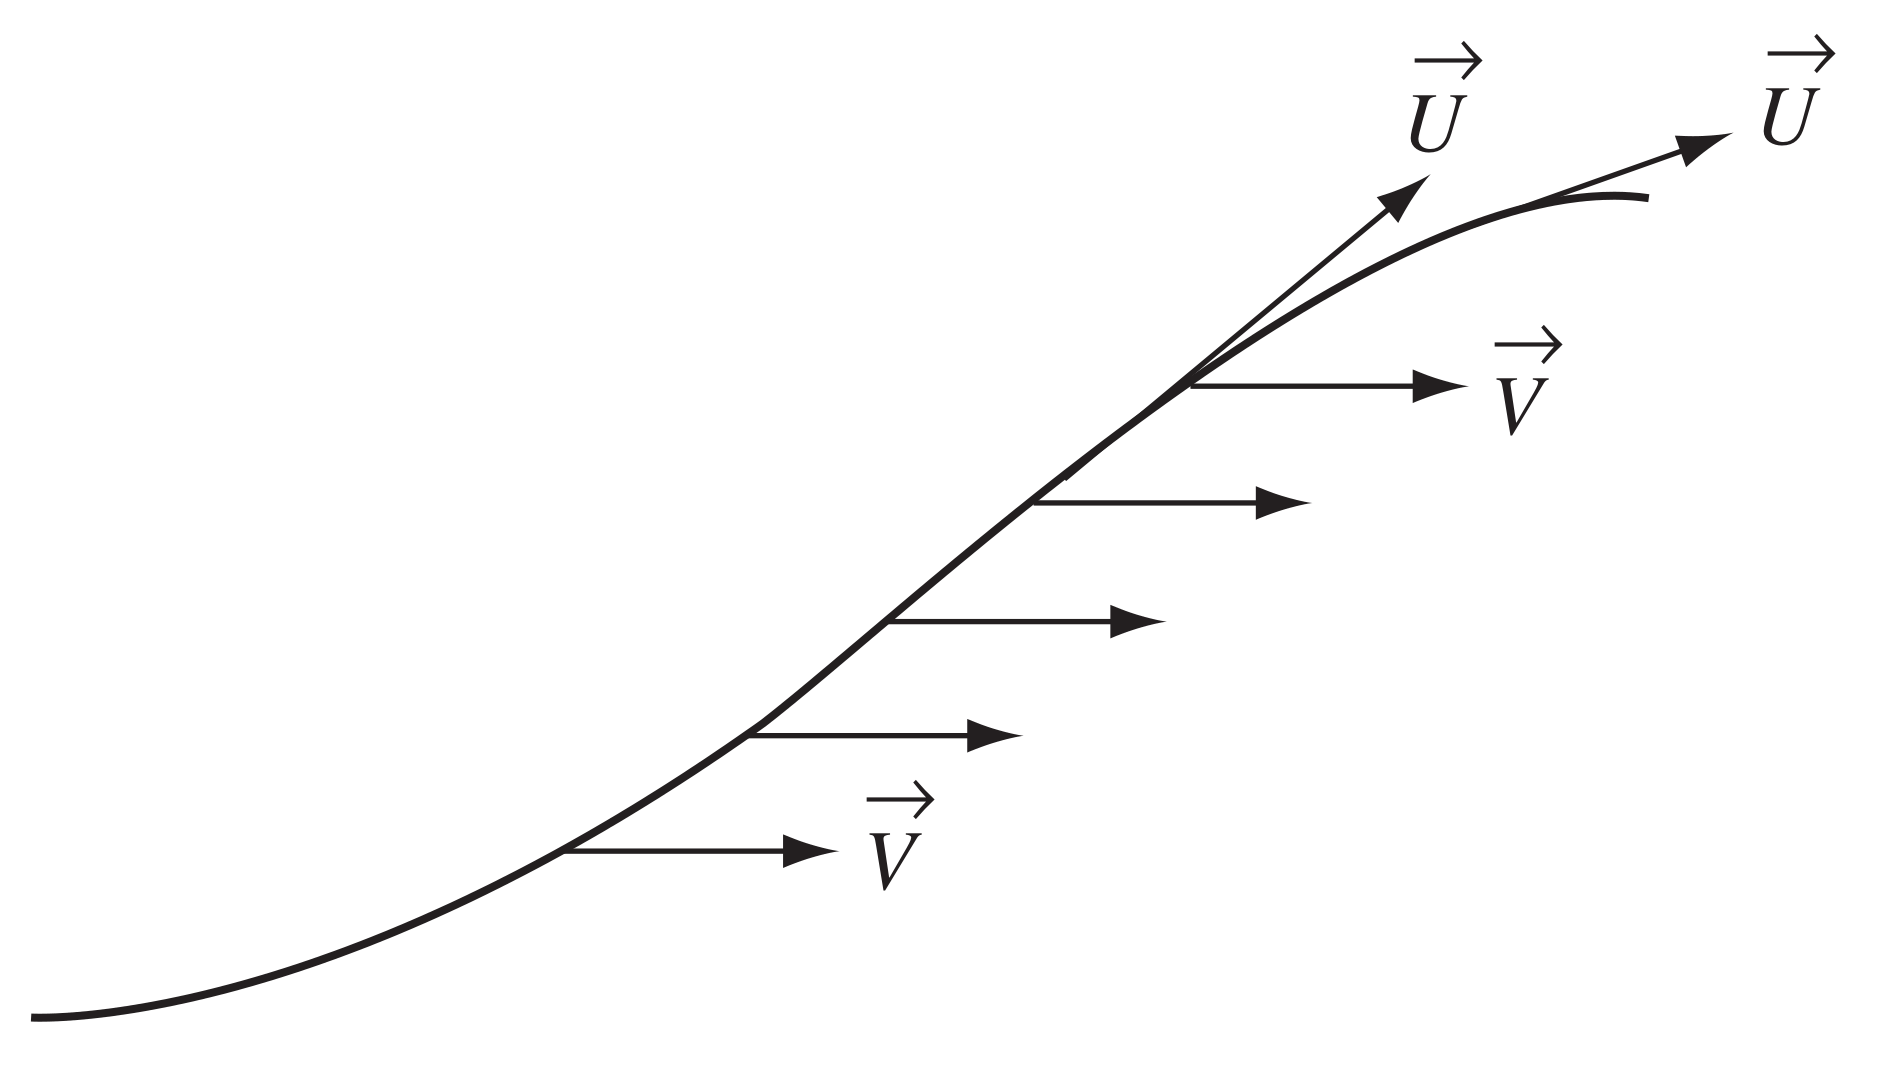
\includegraphics[width=0.6\textwidth]{fig6.4.png}
    \figcaption{\textit{向量$\vec{V}$沿曲线(切向量$\vec{U}$)平行移动。}}
    \label{fig6.4}
}


如果在曲线上相距无穷小两点的向量$\vec{V}$相互平行且长度相等,则称$\vec{V}$沿着该曲线平行移动\footnote{这里“平行移动”是形容词,而前面出现的“平行移动”有时是动词。}(简称平移),这可以很容易地用方程描述。设曲线的参数$\lambda$,切向量$\vec{U} = \rd \vec{x} / \rd \lambda$($\vec{U}$不一定是归一化的),则在曲线任一点$\MP$的局域惯性系中,$\vec{V}$的分量必须沿着$\MP$附近的曲线不变:
\begin{equation}    
    \frac{\rd V^\alpha}{\rd \lambda} = 0 \quad \text{在$\MP$点。}
\label{equ6.46}
\end{equation}
这可以表示为:
\begin{equation}
    \frac{\rd V^\alpha}{\rd \lambda} = U^\beta V\indices{^\alpha_{, \beta}} = U^\beta V\indices{^\alpha_{; \beta}} = 0 \quad \text{在$\MP$点。}
\label{equ6.47}
\end{equation}
其中,第一个等号来自$V^\alpha$沿曲线导数的定义;第二个等号来自局域惯性系中的$\MP$点有$\Gamma\indices{^\alpha_{\mu \nu}} = 0$;第三个等号$U^\beta V\indices{^\alpha_{; \beta}} = 0$是个张量方程,在任意坐标系都成立,因此,\textbf{$\vec{V}$沿着$\vec{U}$平行移动的定义}不依赖于坐标系的形式为:
\begin{shaded}
\begin{equation}
    U^\beta V\indices{^\alpha_{; \beta}} = 0 \quad \Leftrightarrow \quad \frac{\rd}{\rd \lambda} \vec{V} = \nabla_{\vec{U}} \vec{V} = 0.
\label{equ6.48}
\end{equation}
\end{shaded}
其中用到了沿着$\vec{U}$的导数的记号,见\eqref{equ3.67}式。

\subsection*{测地线}
平直空间最重要的曲线是直线。欧几里得公设的其中一条是,两条最初平行的直线延伸下去总保持平行。“延伸”的意思是啥?\textbf{当然不是}意味着“保持两条线之间的距离不变”,否则两条同时掰弯的直线也算作平行了。“延伸”意味着保持最初的方向一直进行下去,更精确地说,曲线下一点的切向量与上一点的切向量平行。实际上,直线是欧几里得空间中\textbf{唯一的}切向量沿自身平行移动的曲线!弯曲空间也可以通过要求\textbf{曲线的切向量沿曲线自身平行移动}以得到“尽量直”的线,这种线称为\textbf{测地线 (geodesics)}:
\begin{shaded}
\begin{equation}
    \{ \vec{U}\ \text{是测地线的切向量} \} \quad \Leftrightarrow \quad \nabla_{\vec{U}} \vec{U} = 0.
\label{equ6.49}
\end{equation}
\end{shaded}
(注意,在局域惯性系中,测地线\textit{是}直的)上式用分量记号写为:
\begin{equation}
    U^\beta U\indices{^\alpha_{; \beta}} = U^\beta U\indices{^\alpha_{, \beta}} + \Gamma\indices{^\alpha_{\mu \beta}} U^\mu U^\beta = 0.
\label{equ6.50}
\end{equation}
设曲线的参数为$\lambda$,则$U^\alpha = \rd x^\alpha / \rd \lambda$以及$U^\beta \partial / \partial x^\beta = \rd / \rd \lambda$:
\begin{shaded}
\begin{equation}
    \frac{\rd}{\rd \lambda} \left( \frac{\rd x^\alpha}{\rd \lambda} \right) + \Gamma\indices{^\alpha_{\mu \beta}} \frac{\rd x^\mu}{\rd \lambda} \frac{\rd x^\beta}{\rd \lambda} = 0.
\label{equ6.51}
\end{equation}
\end{shaded}
Christoffel符号$\Gamma\indices{^\alpha_{\mu \beta}}$是坐标$\{ x^\alpha \}$的已知函数,因此上式是关于$x^\alpha (\lambda)$的非线性(准线性)、二阶微分方程组。在$\lambda = \lambda_0$的初始条件$x_0^\alpha = x^\alpha (\lambda_0)$与$U_0^\alpha = (\rd x^\alpha / \rd \lambda)_{\lambda_0}$给定之后,方程组有唯一解。因此,给定初始位置($x^\alpha_0$)与初始方向($U^\alpha_0$)就确定了唯一的测地线。

回顾一下,如果对参数进行变换,那么从数学上说就得到了不同的曲线(尽管曲线经过的点不变)。设$\lambda$是某测地线的参数(即方程\eqref{equ6.51}成立),如果定义新参数
\begin{equation}
    \phi = a\lambda + b,
\label{equ6.52}
\end{equation}
其中$a, b$是\textbf{常数}(不依赖于曲线上的位置),则$\phi$也是测地线参数,方程\eqref{equ6.51}对$\phi$也成立:
\[
    \frac{\rd^2 x^\alpha}{\rd \phi^2} + \Gamma\indices{^\alpha_{\mu \beta}} \frac{\rd x^\mu}{\rd \phi} \frac{\rd x^\beta}{\rd \phi} = 0.
\]
一般而言,测地线参数$\lambda$\textbf{只有}经过\eqref{equ6.52}式那样的变换之后得到的新参数才仍然是测地线参数,上面的$\lambda, \phi$称为\textbf{仿射 (affine)}参数。如果一条曲线的路径与测地线相同,而它的参数并非仿射参数,则严格说来它不是测地线。

测地线也是任意两点之间的\textbf{极值长度 (extremal length)}曲线:其长度在曲线的一阶微小变化之下的变化量为零。读者一定要尝试证明这个命题,从曲线长度的定义\eqref{equ6.7}式出发,找到固定$\lambda_0, \lambda_1$的极值长度曲线所满足的Euler-Lagrange方程,然后结合\eqref{equ6.32}式证明所导出的极值曲线满足测地线方程\eqref{equ6.51}式,这是个十分有益的练习。此外,读者还可以证明测地线的固有长度是一种仿射参量(见本章习题13-15)。

\section{曲率张量}
\label{sec6.5}

\section{Bianchi恒等式:Ricci张量与Einstein张量}
\label{sec6.6}

\section{Curvature in perspective}
\label{sec6.7}

\section{扩展阅读}
\label{sec6.8}

\section{习题}
\label{sec6.9}